\documentclass[a4paper, 12pt]{article}

\usepackage[english, russian]{babel}
\usepackage[T2A]{fontenc}
\usepackage[utf8]{inputenc}
\usepackage{mathtext}
\usepackage{amsfonts}
\usepackage{ amssymb }
\usepackage{amsmath}
\usepackage{graphics}
\usepackage{graphicx}
\usepackage{wrapfig}
\usepackage{geometry}
\usepackage{float}
\geometry{
	a4paper,
	total={170mm, 257mm},
	left=20mm,
	top=10mm}
	
\title{Лабораторная работа 3.2.2 \\ Резонанс напряжений в последовательном контуре}
\author{Абакшин Василий, Б05-207}
\date{8 ноября 2023 г.}
\newcommand{\E}{\mathcal{E}}
\usepackage{float}
\begin{document}
	\maketitle
	\subsection*{Краткая теория}
	Импеданс последовательного контура:
	\[Z = Z_R + Z_C + Z_L = R + \frac{1}{iwC} + iwL\]
	Ток в цепи:
	\[I = \frac{\E}{Z} = \frac{\E}{R + \frac{1}{iwC} + iwL}\]
	С учетом характеристик цепи: $w_0^2 = \frac{1}{LC}, \ \delta = \frac{R}{2L}$ получаем напряжения на всех элементах:
	\[U_C = IZ_C = \frac{\E}{R + \frac{1}{iwC} + iwL} \cdot \frac{1}{iwC} = \frac{\E}{1 - w^2LC + iwCR} = \frac{\E w_0^2}{w_0^2 - w^2 + 2i\delta w}\]
	\[U_L = IZ_L = \frac{\E w^2}{w^2 - w_0^2 - 2i\delta w}\]
	
	\[U_R = IR = \frac{\E 2i\delta w}{w_0^2 - w^2 + 2i\delta w}\]
	Если контур обладает хорошей добротностью $Q = \frac{w_0}{2\delta}$, то резонансная частота $w_\text{рез} \approx w_0$, на которой в $Q$ раз увеличивается напряжение на конденсаторе и катушке:
	\[U_C = -i\E \frac{w_0}{2\delta} = -i\E Q, \quad U_L = i\E \frac{w_0}{2\delta} = i\E Q, \quad U_R = \E \]
	Напряжения на катушке и конденсаторе находятся в противофазе, и всё напряжение источника находится на активном сопротивлении.\\
	Добротность можно также измерить по амплитудно-частотной характеристике: \[Q = \frac{w_0}{2\Delta w}\] где $2\Delta w$ - ширина резонансной кривой на уровне $U = \frac{U_{\text{рез}}}{\sqrt{2}}$.
	
	\subsection*{Установка}
	Последовательный контур подключен к источнику напряжения, на который подается сигнал с генератора.
	$R_L$ и $R_C$ - активные сопротивления катушки и конденсатора. Напряжения снимаются вольтметрами 1 и 2 со всей цепи и с конденсатора соответственно.
	\begin{figure}[h!]
		\centering
		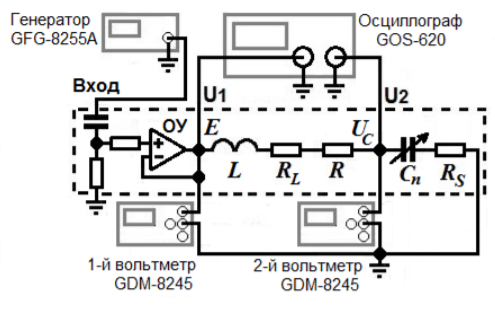
\includegraphics[width = \textwidth]{Цепь}
		\caption{Схема экспериментальной цепи}
	\end{figure}
	\newpage
	\subsection*{Ход работы и обработка результатов}
	\begin{table}[h!]
	\begin{tabular}{|c|c|c|c|c|c|c|c|c|c|c|c|}
		\hline
		$n$ & $C_n$, нФ & \begin{tabular}[c]{@{}c@{}}$f_{0n}$, \\ кГц\end{tabular} & $U_C$, В & $E$, В & \begin{tabular}[c]{@{}c@{}}$L$, \\ мкГн\end{tabular} & $Q$ & \begin{tabular}[c]{@{}c@{}}$\rho$, \\ Ом\end{tabular} & \begin{tabular}[c]{@{}c@{}}$R_{\sum}$, \\ Ом\end{tabular} & \begin{tabular}[c]{@{}c@{}}$R_{S_{\max}}$,\\ Ом\end{tabular} & $R_L$, Ом & $I$, мА \\ \hline
		1 & 25,0 & 31,34 & 4,92 & 0,2 & 1031,58 & 24,61 & 203,13 & 8,25 & 0,203 & 4,60 & 24,22 \\ \hline
		2 & 33,2 & 27,36 & 4,41 & 0,2 & 1019,22 & 22,07 & 175,21 & 7,94 & 0,175 & 4,31 & 25,17 \\ \hline
		3 & 47,5 & 23,00 & 3,84 & 0,2 & 1008,07 & 19,23 & 145,68 & 7,58 & 0,146 & 3,98 & 26,36 \\ \hline
		4 & 57,2 & 21,01 & 3,55 & 0,2 & 1003,21 & 17,79 & 132,43 & 7,45 & 0,132 & 3,86 & 26,81 \\ \hline
		5 & 67,4 & 19,45 & 3,17 & 0,2 & 993,44 & 15,90 & 121,41 & 7,63 & 0,121 & 4,06 & 26,11 \\ \hline
		6 & 82,1 & 17,57 & 3,04 & 0,2 & 999,43 & 15,25 & 110,33 & 7,23 & 0,110 & 3,67 & 27,55 \\ \hline
		7 & 99,6 & 15,99 & 2,81 & 0,2 & 994,68 & 14,10 & 99,93 & 7,08 & 0,099 & 3,53 & 28,12 \\ \hline
		\multicolumn{5}{|c|}{Среднее значение} & 1007,09 & \multicolumn{4}{c|}{--} & 4,00 & -- \\ \hline
		\multicolumn{5}{|c|}{Случайная погрешность} & 13,91 & \multicolumn{4}{c|}{--} & 0,36 & -- \\ \hline
	\end{tabular}
	\caption{Измерение резонансных частот и характеристик контура}
	\end{table}
	Относительный вклад активных потерь на конденсаторах: $\frac{R_{S_{max}}}{R_{\sum}} \leq 2,4 \% $, среднее значение $1,8 \%$. Также полученные данные имеют систематическую погрешность ввиду погрешности вольтметра $\varepsilon_{U_C} = \leq 3\%$ и погрешности измерения резонансной частоты, примем её за $\varepsilon_f = 1 \%$. Тогда получаем следующие относительные систематические погрешности для полученных величин:
	\begin{table}[h!]
		\centering
		\begin{tabular}{|c|c|c|c|c|c|c|}
			\hline
			$L$ & $Q$ & $\rho$ & $R_{\sum}$ & $R_{S_{max}}$ & $R_L$ & $I$ \\ \hline
			2\% & 3\% & 1\% & 3,2\% & 1\% & 6\% & 3,2\% \\ \hline
		\end{tabular}
		\caption{Относительные систематические погрешности величин}
	\end{table}
	
	Также были сняты данные для амплитудно-частотной и фазо-частотной характеристик для емкостей $C_2 = 33,2$ нФ и $C_6 = 82,1$ нФ. Для АЧХ получился следующий график:
	
	\begin{figure}[h]
		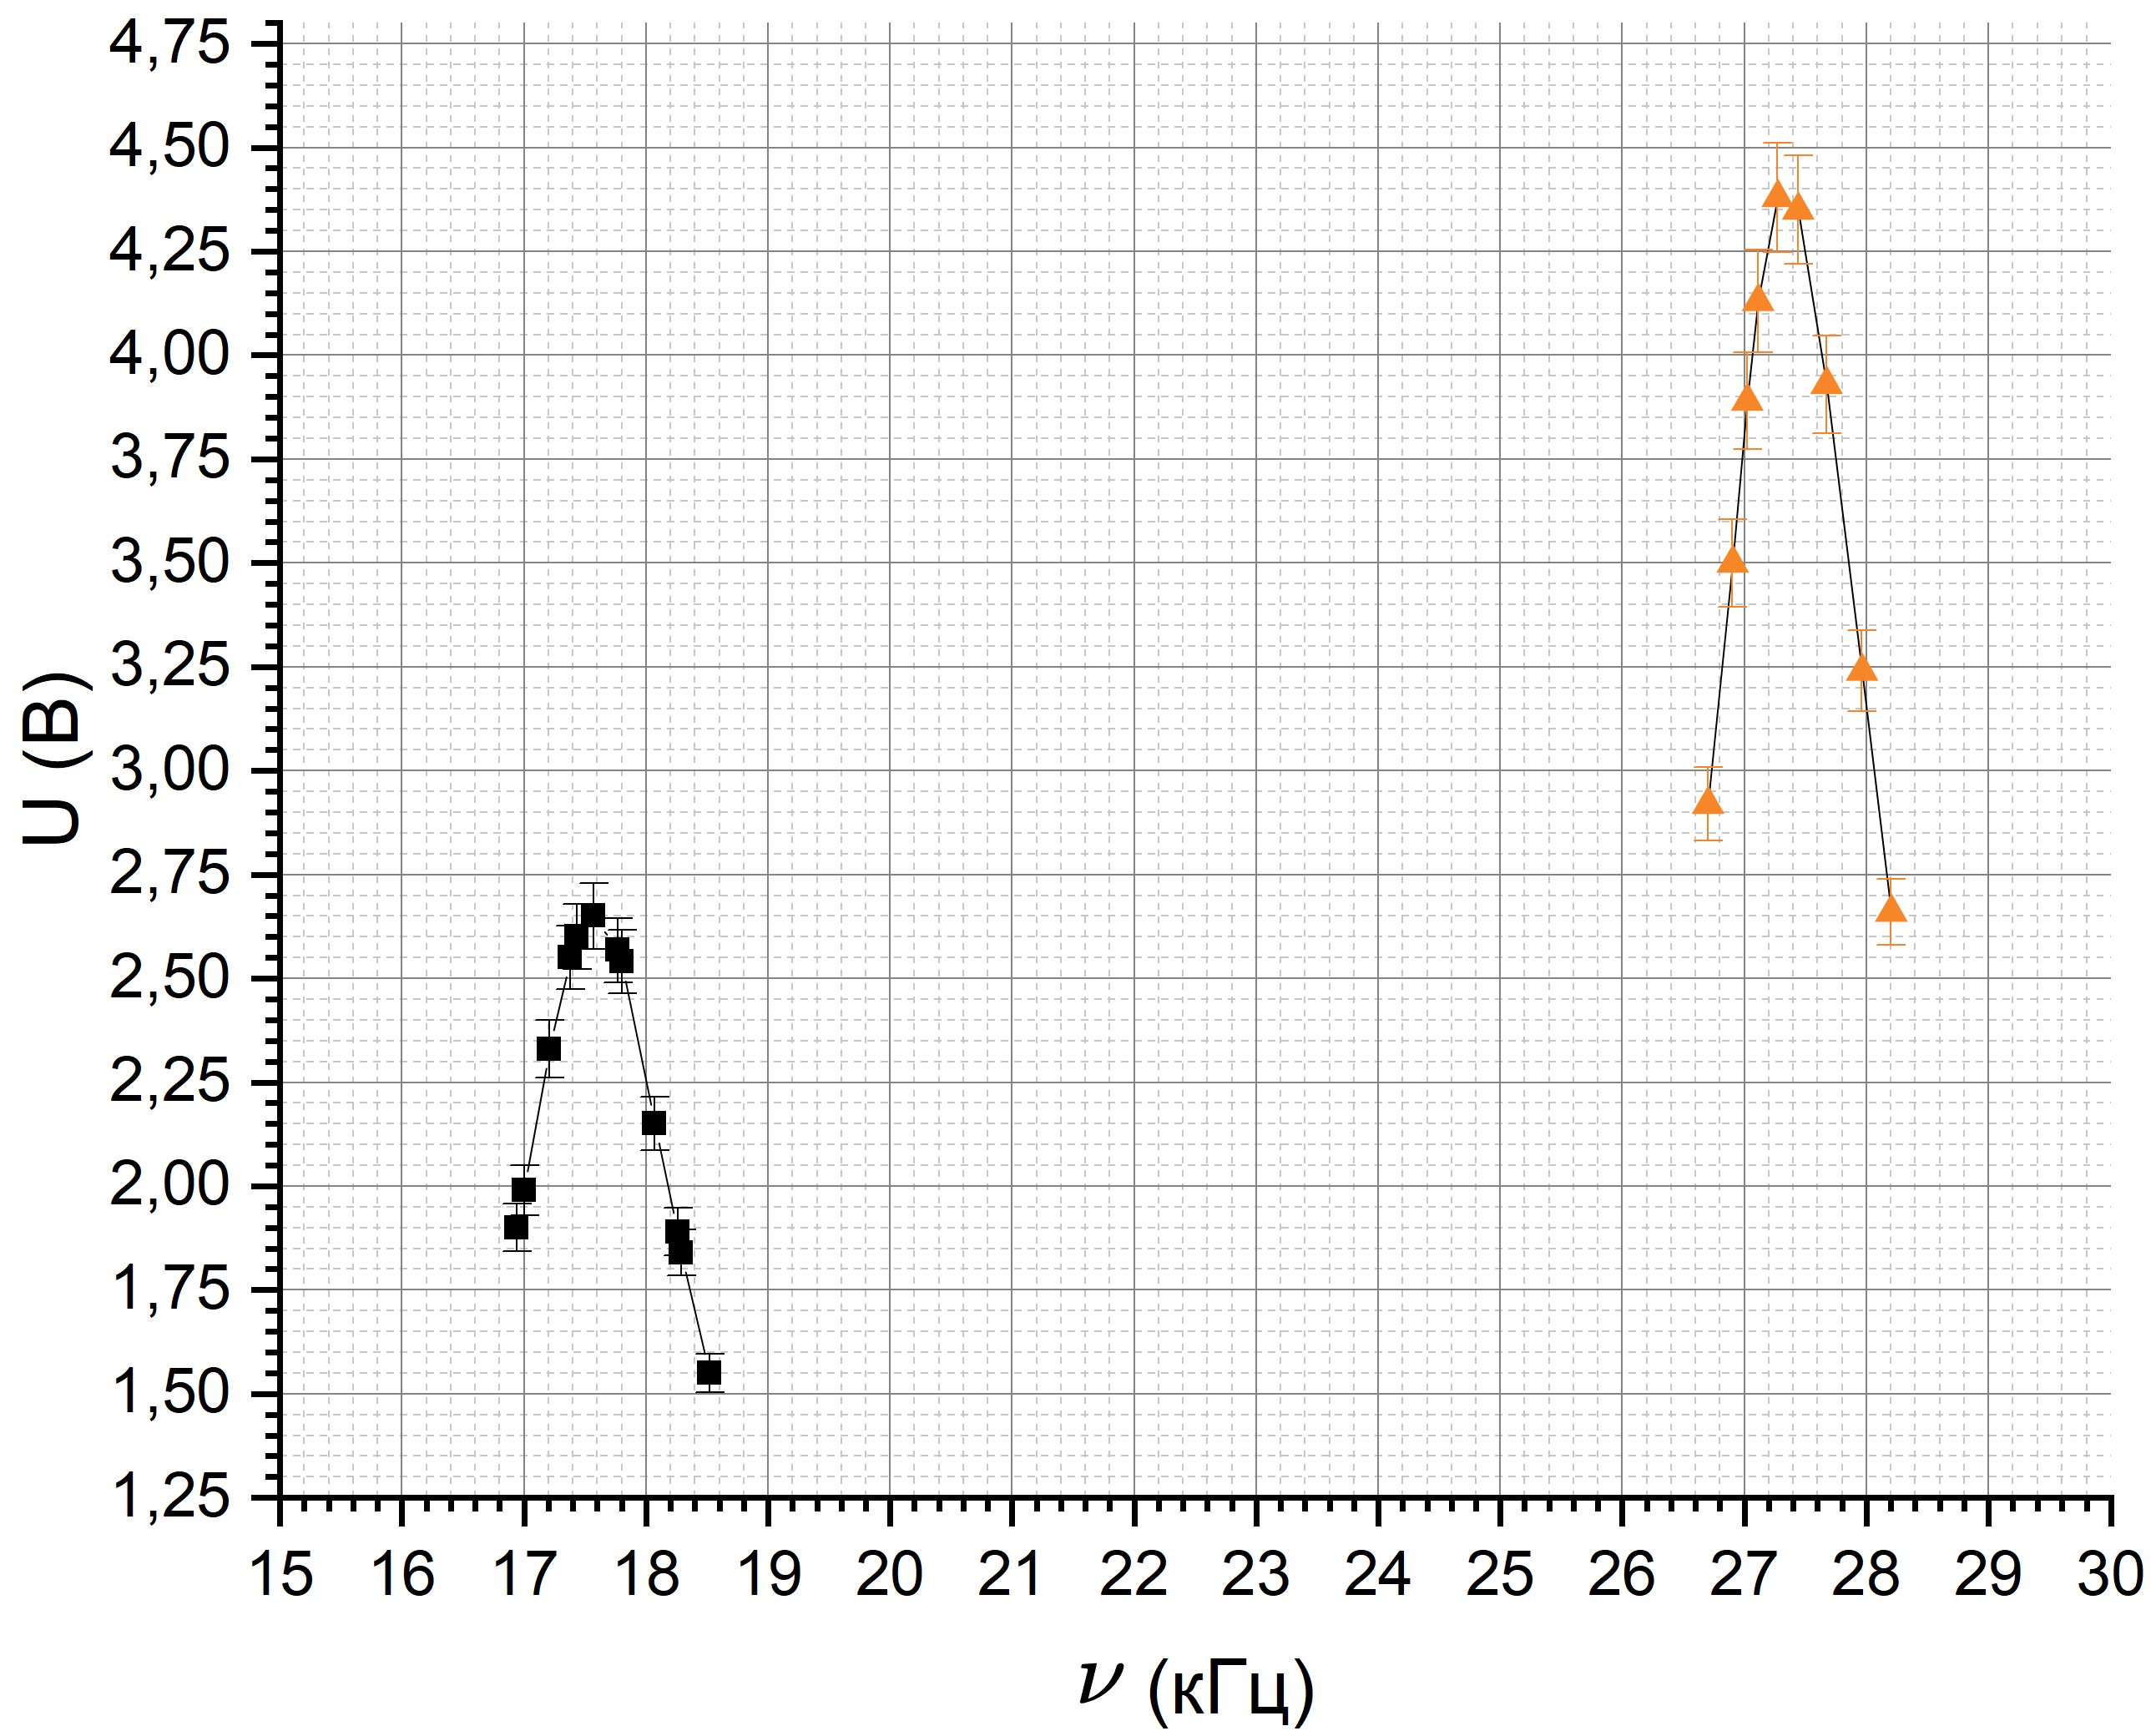
\includegraphics[width = \textwidth]{2AFCH}
		\caption{АЧХ для емкостей $C_2$ (справа) и $C_6$(слева)}
	\end{figure}
	
	Видно, что большей емкости отвечает кривая с большей шириной (так как добротность ниже). Измерим добротности с помощью ширины резонансной кривой на графике в относительном масштабе. Получились следующие значения:
	
	\begin{table}[h]
		\centering
		\begin{tabular}{|c|c|c|c|}
			\hline
			$n$ & $C$, нФ & $\frac{2\Delta \nu}{\nu_0}$ & $Q$ \\ \hline
			2 & 33,2 & 0,0452 & 22,12 \\ \hline
			6 & 82,1 & 0,077 & 12,99 \\ \hline
		\end{tabular}
		\caption{Расчет добротности по ширине АЧХ}
	\end{table}
	
	Рассчитаем также добротность по ФЧХ: измерим ширину кривой, которая ограничивается значениями $\frac{\Delta \phi}{\pi}$ от 0,25 до 0,75, получим следующие значения добротностей:
	
	\begin{figure}[H]
		\centering
		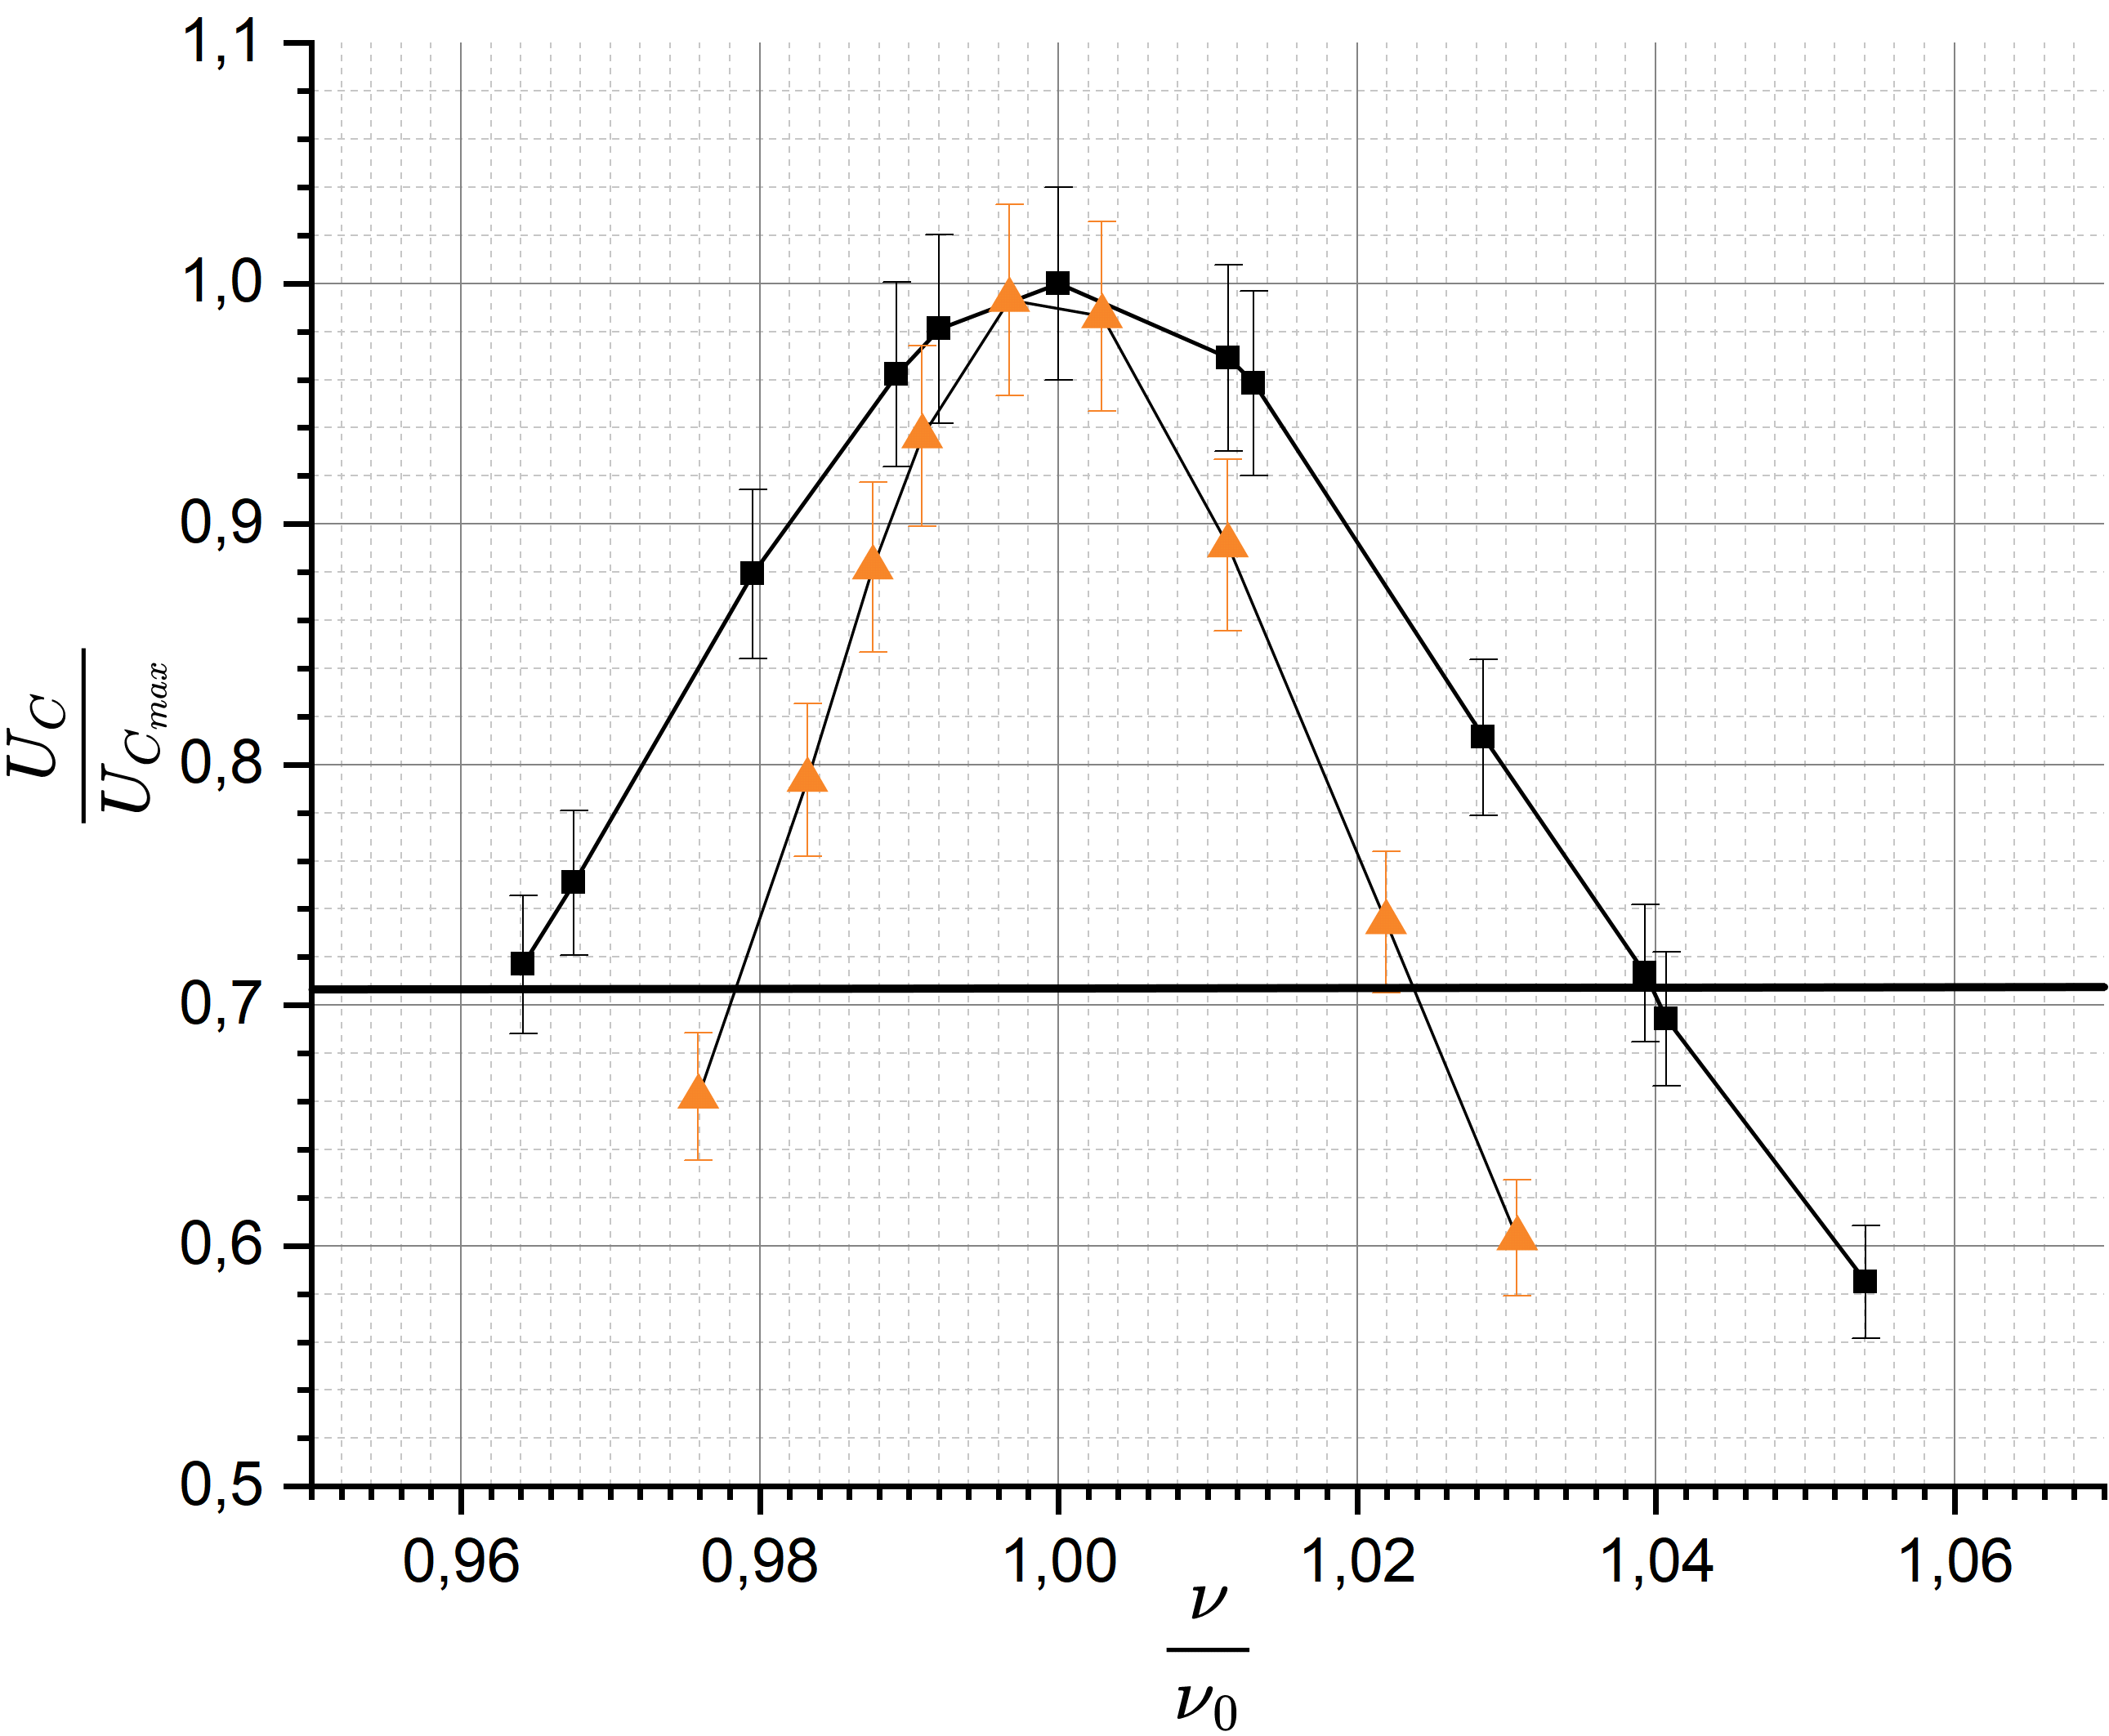
\includegraphics[width = 0.85\textwidth, height = 0.44\textheight]{LinedAFCH}
		\caption{АЧХ в относительном масштабе}
	\end{figure}
	
	\begin{figure}[H]
		\centering
		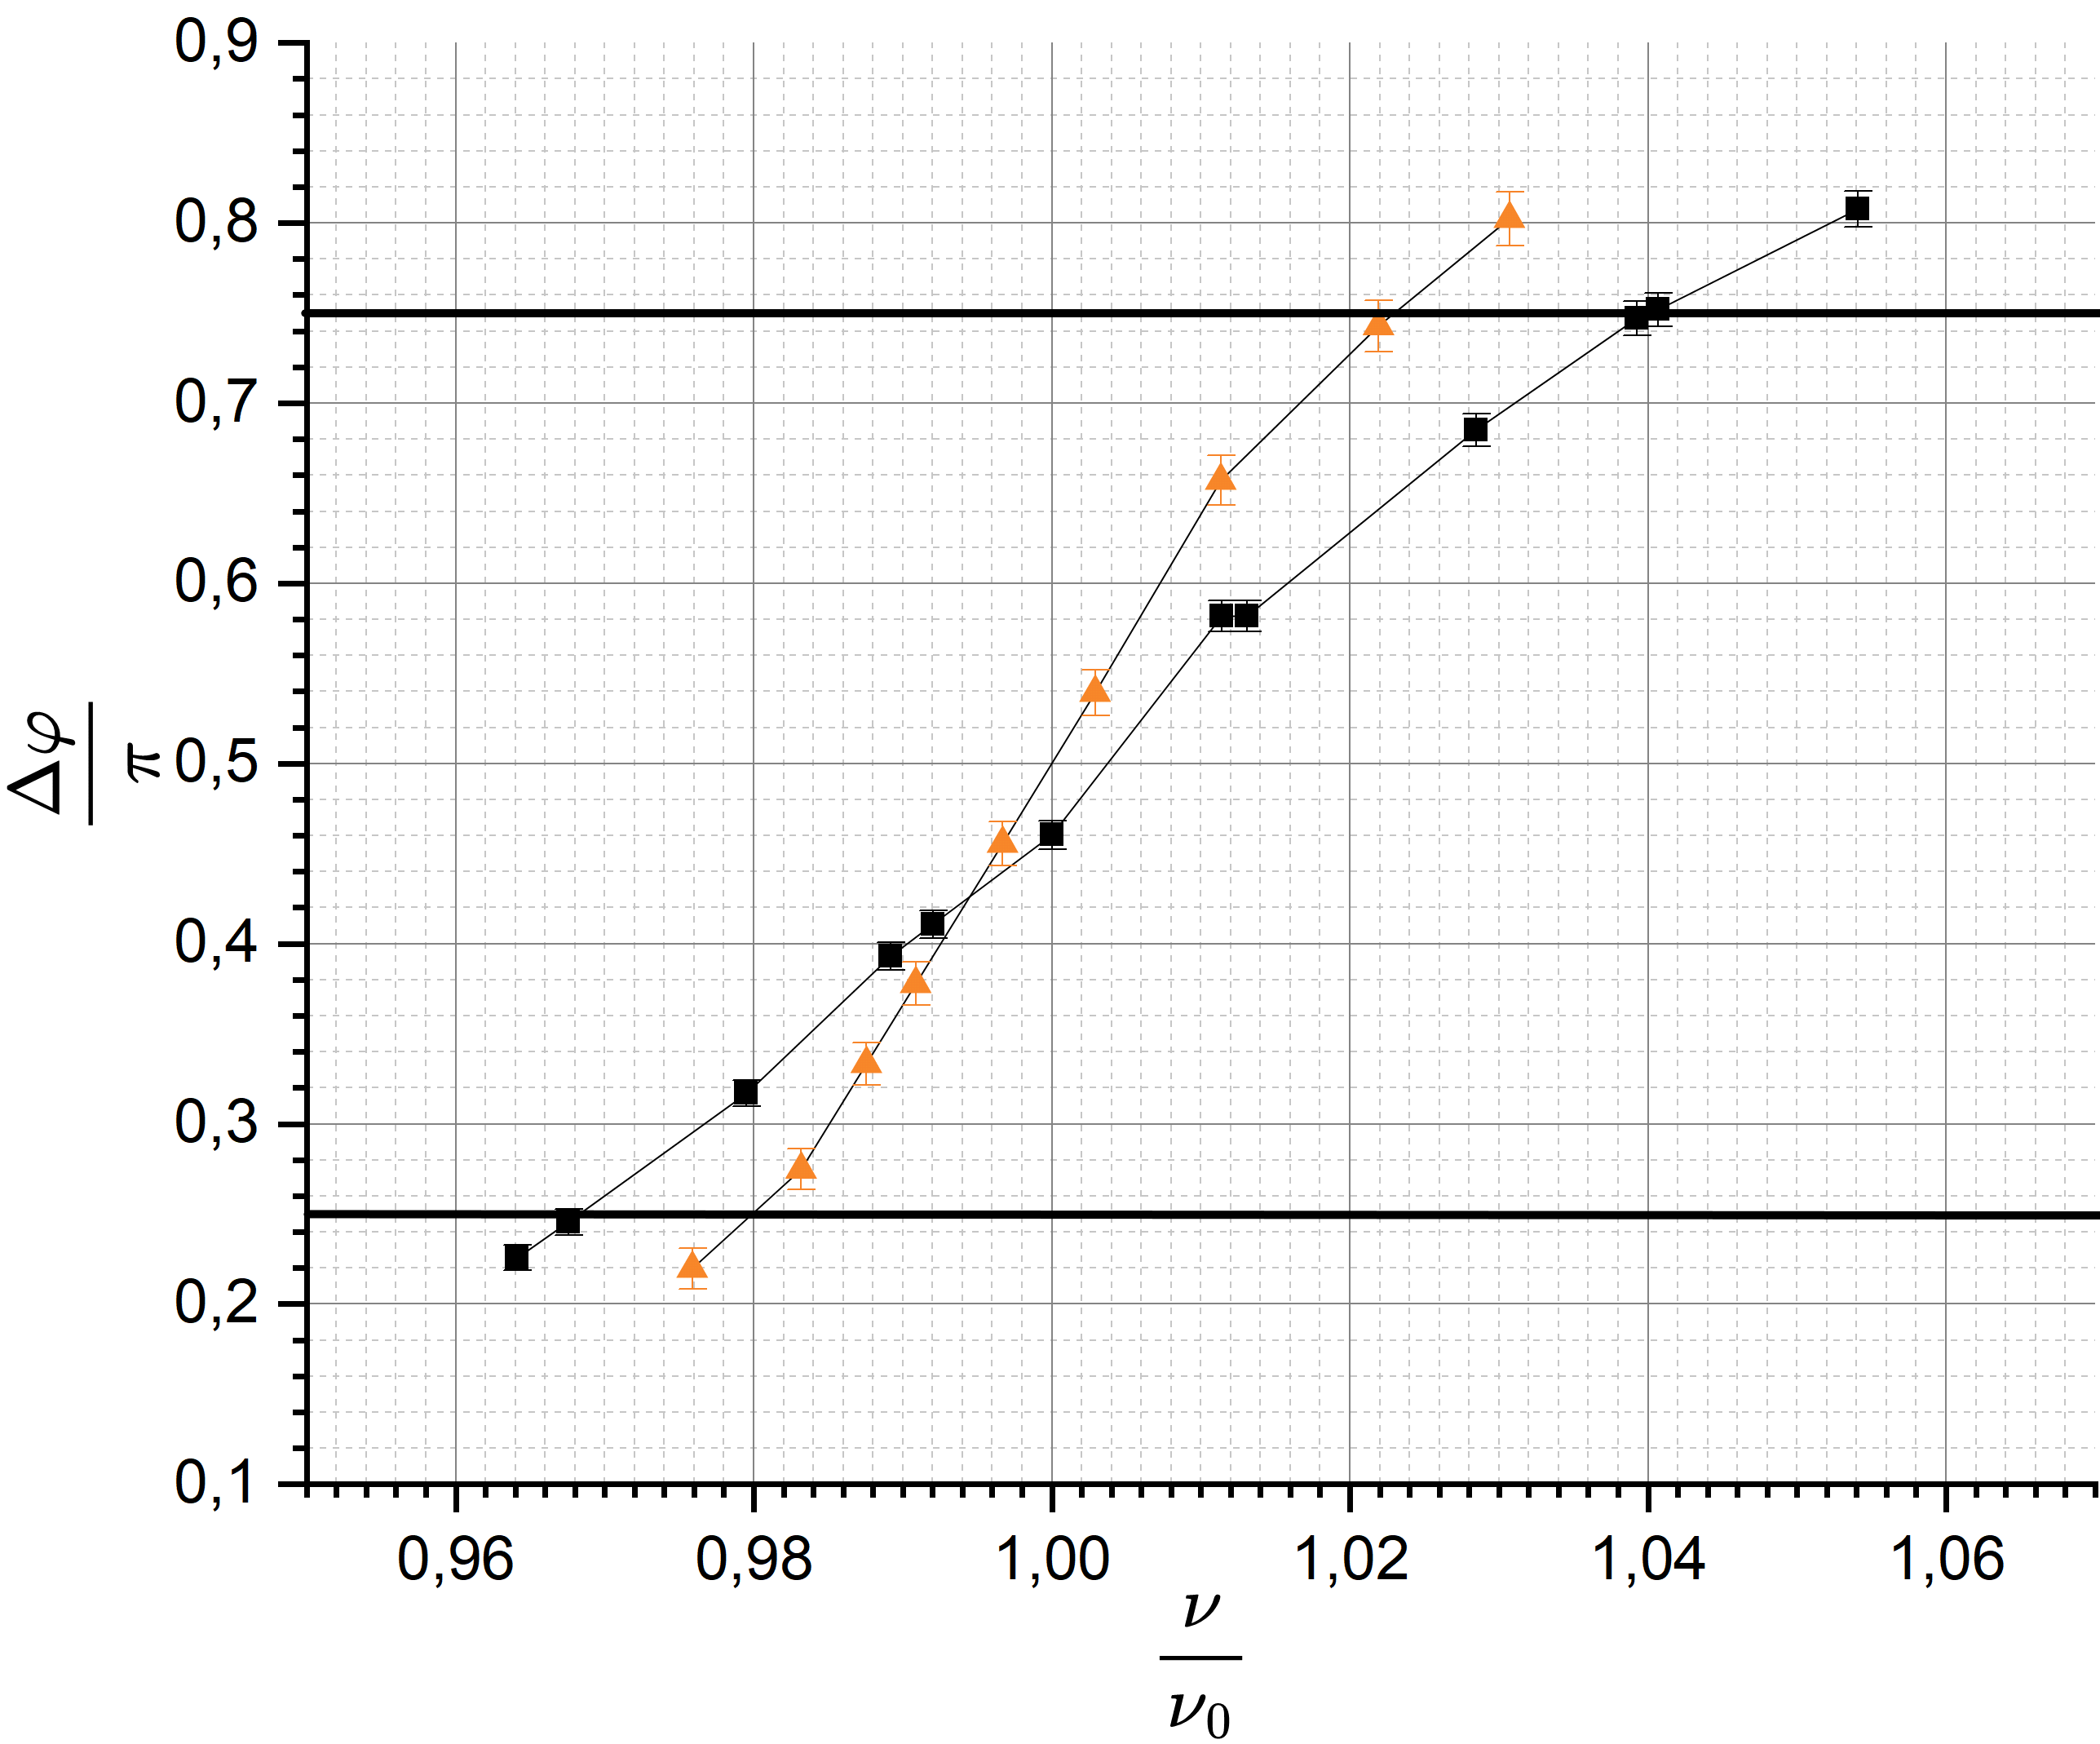
\includegraphics[width = 0.85\textwidth, height = 0.44\textheight]{LinedPhFCH}
		\caption{ФЧХ в относительном масштабе}
	\end{figure}
	
	\begin{table}[h]
		\centering
		\begin{tabular}{|c|c|c|c|}
			\hline
			$n$ & $C$, нФ & $\frac{2\Delta \nu}{\nu_0}$ & $Q$ \\ \hline
			2 & 33,2 & 0,043 & 23,26 \\ \hline
			6 & 82,1 & 0,072 & 13,89 \\ \hline
		\end{tabular}
		\caption{Расчет добротности по ширине ФЧХ}
	\end{table}
	
	Построим теперь график зависимость $R_L(\nu)$.
	
	\begin{figure}[h]
		\centering
		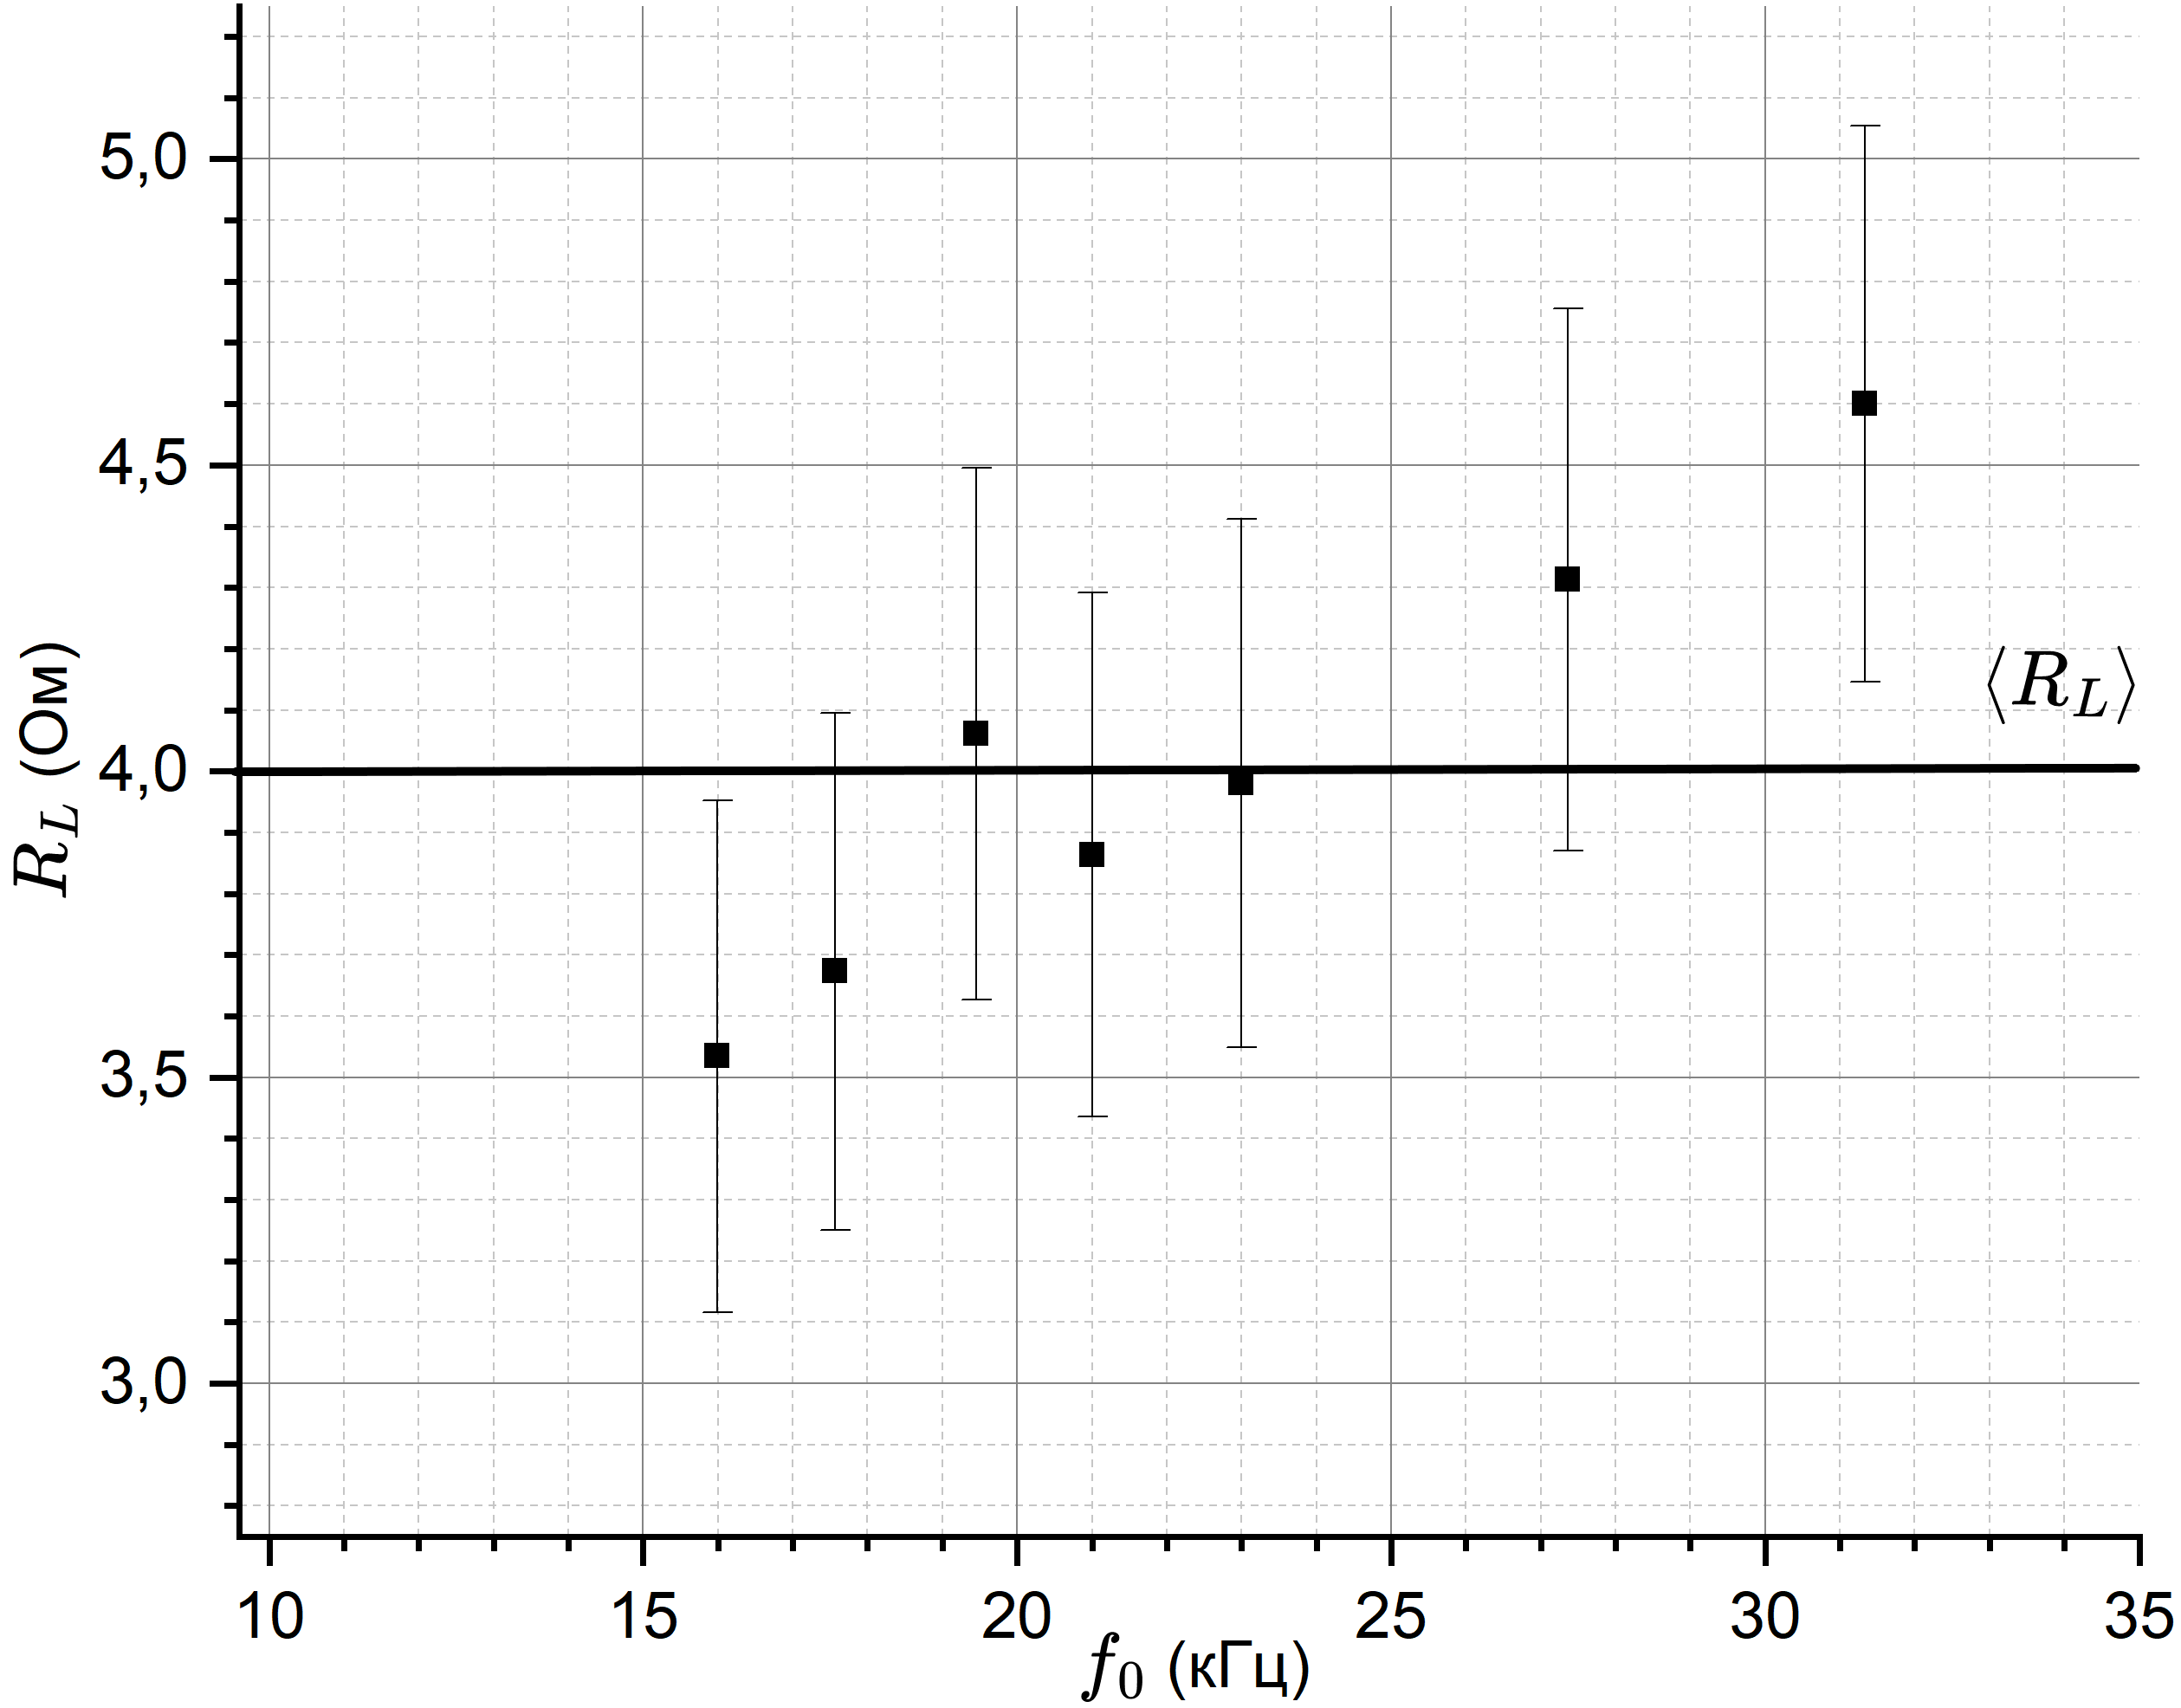
\includegraphics[width = \textwidth]{LinedR_L}
		\caption{Зависимость $R_L(\nu)$}
	\end{figure}
	
	Значения отклоняются от среднего достаточно сильно, прослеживается почти линейная зависимость от частоты. Из возможных причин можно выделить влияние скин-эффекта, из-за которого ток вытесняется на поверхность проводника и течет по меньшему сечению.
	\newpage
	
	\begin{wrapfigure}{l}{0,35\textwidth}
		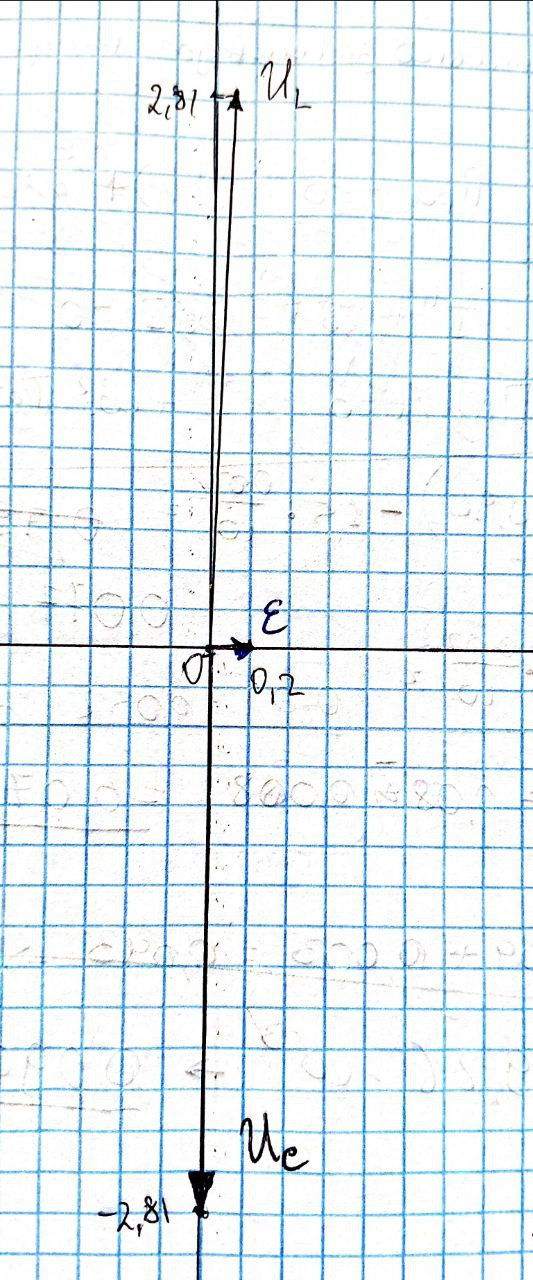
\includegraphics[height = 0.5\textheight]{Vector_diagram}
		\caption{Векторная диаграмма напряжений}
	\end{wrapfigure}
	
	Требуется также построить векторные диаграммы токов и напряжений при резонансе для контура с минимальной добротностью. Так как контур последовательный, то токи будут находится на всех элементах в одной фазе. А вот с напряжением ситуация другая: напряжения на конденсаторе и катушке почти в противофазе, причем из напряжение на катушке опережает $\E$ на $\frac{\pi}{2}$, а напряжение на конденсаторе отстаёт от $\E$ на $\frac{\pi}{2}$.
	$U_L$ расположена под углом $\varphi = 87,6$\textdegree, так как на катушке есть еще активное сопротивление $R_L$. $\tg{\varphi}$ можно рассчитать как $\frac{U_{C_{\text{рез}}}}{IR_L}$. 
	
	\subsection*{Выводы}
	
	В данной лабораторной работе был исследован резонанс напряжений в последовательном контуре и вычислены добротности контуров с различными значениями емкости несколькими способами. Так как получившиеся ФЧХ и АЧХ не очень точны ввиду небольшого числа точек и их неравномерности, то погрешность при расчете добротности через ширину резонансных кривых достаточно велика. Однако, рассчет по АЧХ получился достаточно точным в случае контура с $C_2$. В любом случае, это явно не лучший способ измерять добротность контура, гораздо точнее измерение по формулам через параметры контура. 
	
	Было замечено, что активное сопротивление $R_L$ катушки не является постоянным и линейно растет с частотой. Объяснение этому, скорее всего, кроется в скин-эффекте. 
\end{document}